\chapter{Validation}
\label{chap:validation}
The aim of this work was to develop an academic records registry leveraging blockchain technologies, providing students and universities with a reliable system to store and share academic data, thus updating the standard for information management. To create this system, we developed several on-chain and off-chain components that interact to form the \gls{ew} solution. System validation was conducted by testing all components and analysing the results provided by the testing environment.

\section{Components Validation}
The goal of the components validation was to verify whether all the system functionalities, as outlined in \cref{chap:requirements}, had been properly implemented. To perform this verification, we carried out various system-level tests focusing on the interaction among components.

The tests were conducted in the local testing environment, with the Ethereum node configured as explained in \cref{sec:developmentEnvironment}. Given that all elements of the \gls{ew} solution are tightly integrated and designed to work in synergy, the most effective validation approach was to test them as a cohesive unit, specifically, by validating the \gls{sdk} and the browser extension together.

The \gls{sdk} functionalities were tested through the \gls{cli}, using its \gls{ui} to select and execute various operations. The browser extension instead was tested using the Chrome browser, replicating the experience of student users. After performing operations such as the student registration and enrolment via the \gls{cli}, we used the resulting student credentials to log into the extension and verify the data stored in student's academic wallet. Through these tests, we confirmed that all \glspl{fr} were fulfilled for both the \gls{sdk} and the browser extension.

These functional tests revealed a few bugs in system behaviour. For instance, while testing data input through the \gls{cli}, we encountered an issue with date handling: since dates are stored as unsigned timestamps, any date before January 1, 1970, was rejected by the smart contracts, causing transactions to fail. As a result, we implemented additional checks in the off-chain components to validate and restrict date inputs to compatible values. We also noticed occasional graphical glitches in the browser extension. In some cases, a student’s academic record was correctly retrieved but not displayed in the interface. The data would appear only after switching views, for example, from the wallet page to the personal information page.  These issues are likely caused by imperfect handling of the extension’s internal state management and have been noted for future refinement.

\section{Transactions Analysis}
One of the features provided by the local Hardhat node used to test our on-chain components is the ability to analyse transactions. As shown in \cref{fig:exampleTransaction}, Hardhat enables inspection of each transaction and its related information, including the sender and receiver addresses, the amount of \gls{eth} transferred, the computational effort consumed (gas used), and the hash of the block that contains the transaction.
\begin{figure}
  \centering
  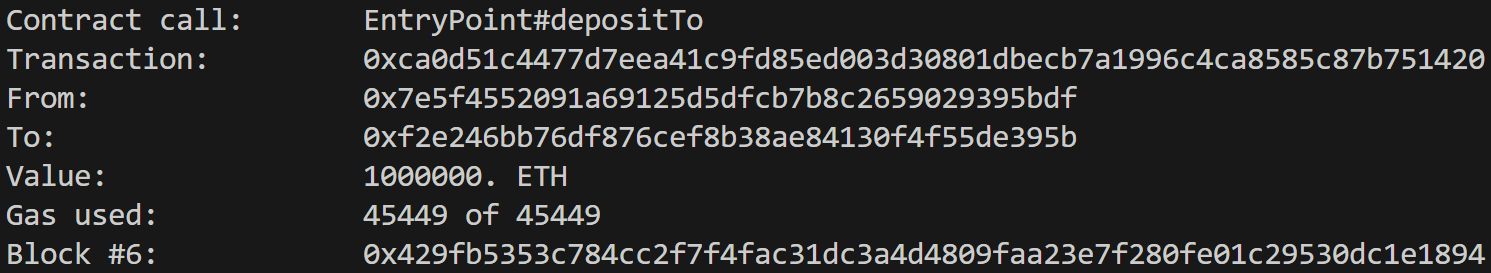
\includegraphics[width=0.9\textwidth]{figures/hardhatExample.png}
  \caption[Transaction information from the local Hardhat node]{Transaction information from the local Hardhat node}
  \label{fig:exampleTransaction}
\end{figure}

Using this data, we analysed the cost of transactions to assess whether the proposed solution is compatible with real-world usage. We did not give significant attention to transaction waiting times in our tests due to the limitations of a local environment. Since the node was not shared with other users and only \gls{ew}-related transactions were processed, transaction delays and congestion were not representative of a real public blockchain scenario.

To convert gas costs into traditional currencies, we used gas prices from online gas trackers\footnote{\url{https://etherscan.io/gastracker} and \url{https://polygonscan.com/gastracker}} and token exchange rates retrieved from an online converter\footnote{\url{https://www.coinbase.com/it/converter}}. The conversion values are summarized in \cref{tab:gasConversions}. Gas prices are expressed in Gwei, a standard unit where 1 Gwei corresponds to $10^{-9}$ \gls{eth} or POL.

\begin{table}
\centering
\caption{Gas prices and exchange rates for Ethereum and Polygon networks}
\label{tab:gasConversions}
\begin{tabular}{|p{0\linewidth}|p{0\linewidth}|p{0.185\linewidth}|p{0.23\linewidth}|p{0.23\linewidth}|}
\hline
\multicolumn{1}{|c|}{\textbf{Network}} & \multicolumn{1}{|c|}{\textbf{Token}} & \textbf{Gas Price (Gwei)} & \textbf{Exchange rate (EUR)} & \textbf{Exchange rate (NOK)} \\
\hline
Ethereum & \gls{eth} & 2 & 2,303.31 & 26,557.16 \\
\hline
Polygon & POL & 30 & 0.19 & 2.19 \\
\hline
\end{tabular}
\end{table}

All transaction data collected during validation are presented in \cref{tab:systemCosts}. In particular, by analysing the distribution diagrams in \cref{fig:operationCosts}, we observe that the costs are relatively contained, with the most frequent cost around 0.5 EUR (5.7 NOK) on the Ethereum network and 0.0001 EUR (0.0012 NOK) on the Polygon network. These diagrams exclude the deployment costs of the four initial smart contracts, StudentsRegister, StudentDeployer, and Paymaster, as these would typically be deployed only once in a real-world scenario and would therefore represent outliers in our analysis.

\begin{table}
\centering
\caption{Gas costs and fiat currency equivalents for EduWallet smart contract operations on Ethereum and Polygon networks.}
\label{tab:systemCosts}
\begin{tabular}{|c|p{0.20\linewidth}|p{0.11\linewidth}|p{0.115\linewidth}|p{0.115\linewidth}|p{0.095\linewidth}|p{0.095\linewidth}|}
\hline
 & \multicolumn{1}{|c|}{\textbf{Operation}} & \multicolumn{1}{|c|}{\textbf{Gas used}} & \multicolumn{2}{c|}{\textbf{Ethereum}} & \multicolumn{2}{c|}{\textbf{Polygon}} \\
\cline{4-7}
& & & \multicolumn{1}{|c|}{\textbf{EUR}} & \multicolumn{1}{|c|}{\textbf{NOK}} & \multicolumn{1}{|c|}{\textbf{EUR}} & \multicolumn{1}{|c|}{\textbf{NOK}} \\
\hline
1 & Deploy 4 core contracts & 5775926 & 26.6075 & 306.7844 & 0.0329 & 0.3796 \\
\hline
2 & Register university & 937412 & 4.3183 & 49.7900 & 0.0053 & 0.0616 \\
\hline
3 & Register student & 3050503 & 14.0525 & 162.0254 & 0.0174 &	0.2005 \\
\hline
4 & Enrol in one course & 228660 & 1.0533 & 12.1451 & 0.0013 & 0.0150 \\
\hline
5 & Enrol in two courses & 335233 & 1.5443 & 17.8057 & 0.0019 & 0.0220 \\
\hline
6 & Evaluate one course & 141137 & 0.6502 & 7.4964 & 0.0008 & 0.0093 \\
\hline
7 & Evaluate two courses & 106053 & 0.4885 & 5.6329 & 0.0006 & 0.0070 \\
\hline
8 & Request permission & 196625 & 0.9058 & 10.4436 & 0.0011 & 0.0129 \\
\hline
9 & Grant permission & 203678 & 0.9383 & 10.8182 & 0.0012 & 0.0134 \\
\hline
10 & Revoke permission & 87306 & 0.4022 & 4.6372 & 0.0005 & 0.0057 \\
\hline
\end{tabular}
\end{table}

For the remaining transactions, as expected, the costs on the Ethereum network are significantly higher, approximately 800 times, compared to those on the Polygon network. For instance, registering a student, which involves deploying a dedicated smart contract, costs approximately 14 EUR (161 NOK) on Ethereum, while on Polygon, the same operation costs about 0.02 EUR (0.23 NOK). Despite the higher costs on Ethereum, the overall expenses of our system remain compatible with real-world usage. For example, considering the academic career of a typical student completing 40 courses, the total wallet management cost would amount to roughly 80 EUR (922 NOK) on Ethereum and only 1.30 EUR (15.00 NOK) on Polygon.   

An important optimization enabled by our system is the ability to enrol in and evaluate multiple courses within a single transaction. This feature significantly improves cost-efficiency compared to processing each course in a separate transaction.

\begin{figure}
    \centering
    \begin{subfigure}{0.99\textwidth}
      \centering
      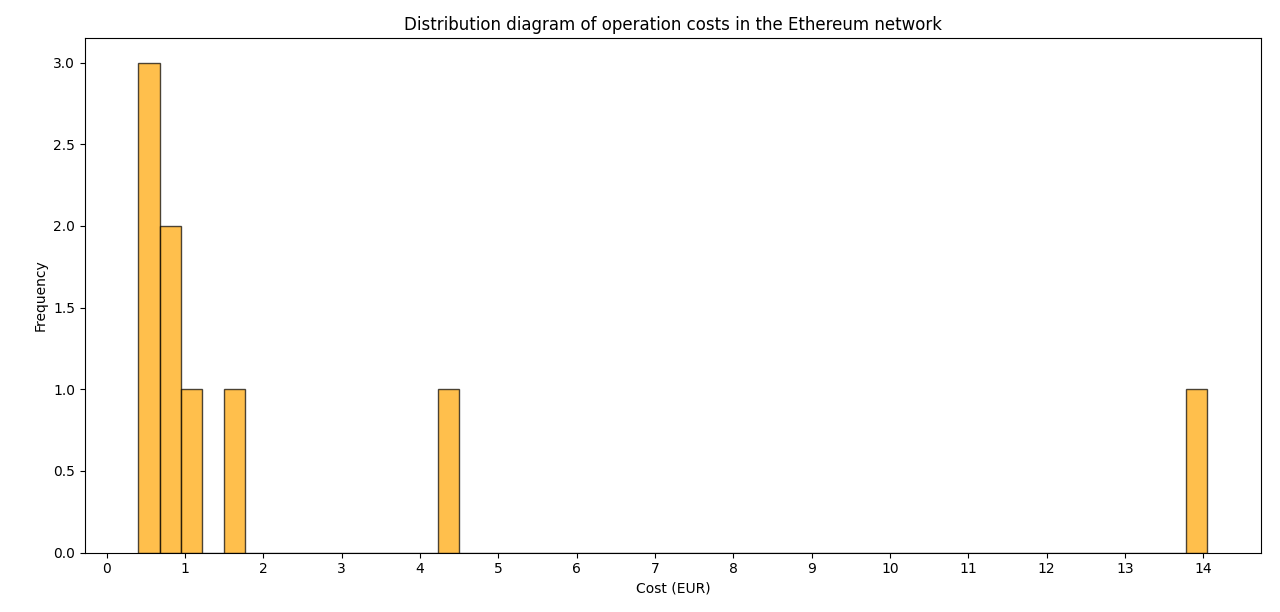
\includegraphics[width=\textwidth]{figures/ethCosts.png}
      \caption{Distribution diagram of operation costs in the Ethereum network}
      \label{fig:ethCosts}
    \end{subfigure}
    \hfill
    \begin{subfigure}{0.99\textwidth}
      \centering
      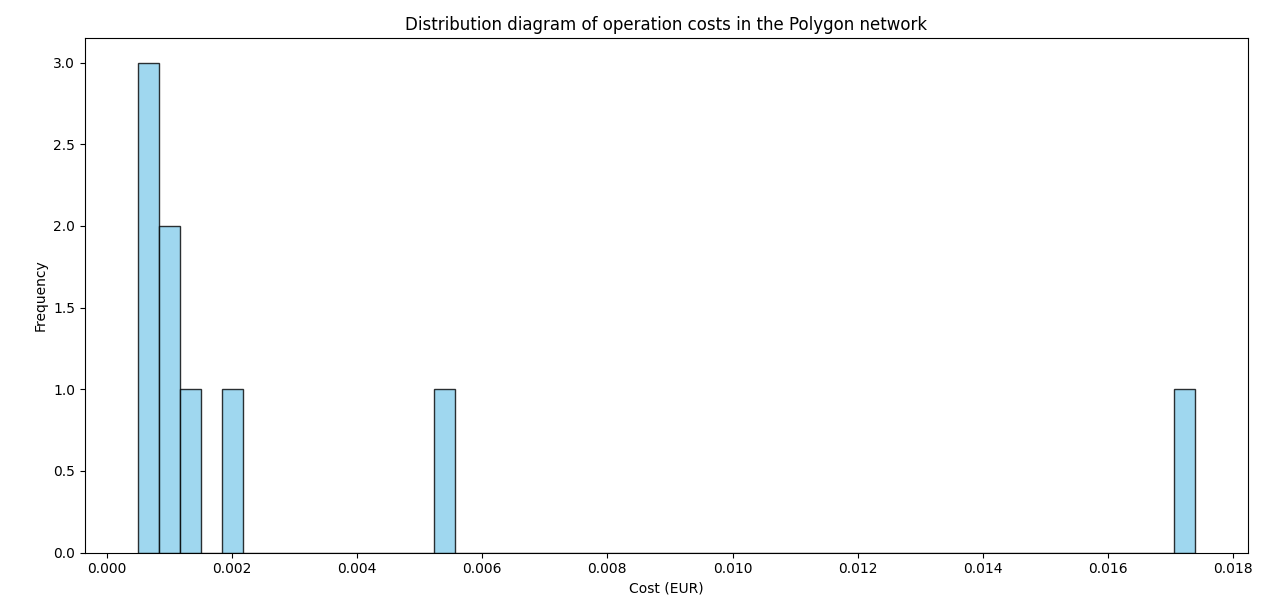
\includegraphics[width=\textwidth]{figures/polCosts.png}
      \caption{Distribution diagram of operation costs in the Polygon network}
      \label{fig:polCosts}
    \end{subfigure}
    \caption[Distribution diagram of operation costs in Ethereum and Polygon]{Distribution diagrams of the cost to execute EduWallet operations in Ethereum and Polygon networks.}
    \label{fig:operationCosts}
\end{figure}

In conclusion, the validation demonstrates that our system satisfies all the \glspl{fr} and \glspl{nfr} outlined in \cref{chap:requirements}. Furthermore, the operational costs of \gls{ew} remain modest, particularly when considering deployment on the Polygon network, which offers significantly lower transaction fees compared to the Ethereum main network.